We shall have a look at groups from the point of view of symmetry operations and then formalize the definition for abstract operations.\\
Say we want to study the symmetry elements of a planar equilateral triangle. First let us label the vertices of the traingle as $A$, $B$ and $C$. Studying the symmetry operations is almost like studying the permissible permutations of $A$, $B$ and $C$ around the vertices of the given triangle. Pictorially, we can have the following symmetry operations:\\
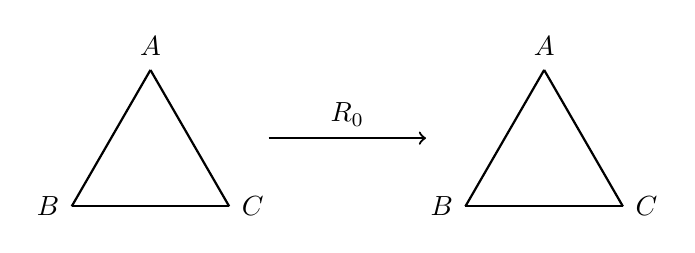
\begin{tikzpicture}
	\draw (1,2.032) node{$A$};
	\draw (-0.3,0) node{$B$};
	\draw (2.3,0) node{$C$};
	\draw (6,2.032) node{$A$};
	\draw (4.7,0) node{$B$};
	\draw (7.3,0) node{$C$};
	\draw (3.5,1.166) node{$R_0$};
	\draw[thick](0,0)--(1,1.732); 
	\draw[thick](0,0)--(2,0);
	\draw[thick](1,1.732)--(2,0);
	\draw[thick,->](2.5,0.866)--(4.5,0.866);
	\draw[thick](5,0)--(6,1.732);
	\draw[thick](5,0)--(7,0);
	\draw[thick](6,1.732)--(7,0);
\end{tikzpicture}
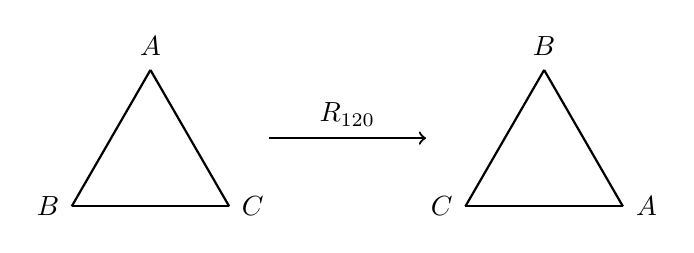
\begin{tikzpicture}
	\draw (1,2.032) node{$A$};
	\draw (-0.3,0) node{$B$};
	\draw (2.3,0) node{$C$};
	\draw (6,2.032) node{$B$};
	\draw (4.7,0) node{$C$};
	\draw (7.3,0) node{$A$};
	\draw (3.5,1.166) node{$R_{120}$};
	\draw[thick](0,0)--(1,1.732); 
	\draw[thick](0,0)--(2,0);
	\draw[thick](1,1.732)--(2,0);
	\draw[thick,->](2.5,0.866)--(4.5,0.866);
	\draw[thick](5,0)--(6,1.732);
	\draw[thick](5,0)--(7,0);
	\draw[thick](6,1.732)--(7,0);
\end{tikzpicture}
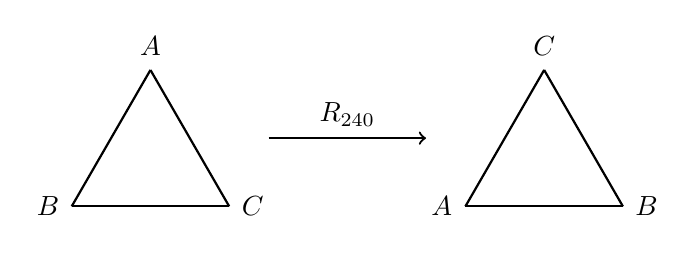
\begin{tikzpicture}
	\draw (1,2.032) node{$A$};
	\draw (-0.3,0) node{$B$};
	\draw (2.3,0) node{$C$};
	\draw (6,2.032) node{$C$};
	\draw (4.7,0) node{$A$};
	\draw (7.3,0) node{$B$};
	\draw (3.5,1.166) node{$R_{240}$};
	\draw[thick](0,0)--(1,1.732); 
	\draw[thick](0,0)--(2,0);
	\draw[thick](1,1.732)--(2,0);
	\draw[thick,->](2.5,0.866)--(4.5,0.866);
	\draw[thick](5,0)--(6,1.732);
	\draw[thick](5,0)--(7,0);
	\draw[thick](6,1.732)--(7,0);
\end{tikzpicture}
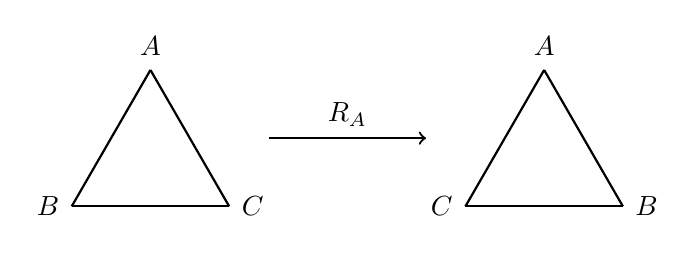
\begin{tikzpicture}
	\draw (1,2.032) node{$A$};
	\draw (-0.3,0) node{$B$};
	\draw (2.3,0) node{$C$};
	\draw (6,2.032) node{$A$};
	\draw (4.7,0) node{$C$};
	\draw (7.3,0) node{$B$};
	\draw (3.5,1.166) node{$R_A$};
	\draw[thick](0,0)--(1,1.732); 
	\draw[thick](0,0)--(2,0);
	\draw[thick](1,1.732)--(2,0);
	\draw[thick,->](2.5,0.866)--(4.5,0.866);
	\draw[thick](5,0)--(6,1.732);
	\draw[thick](5,0)--(7,0);
	\draw[thick](6,1.732)--(7,0);
\end{tikzpicture}
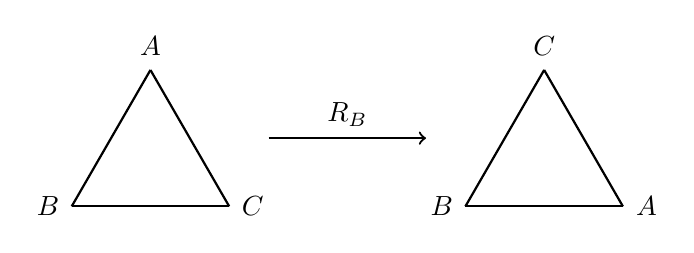
\begin{tikzpicture}
	\draw (1,2.032) node{$A$};
	\draw (-0.3,0) node{$B$};
	\draw (2.3,0) node{$C$};
	\draw (6,2.032) node{$C$};
	\draw (4.7,0) node{$B$};
	\draw (7.3,0) node{$A$};
	\draw (3.5,1.166) node{$R_B$};
	\draw[thick](0,0)--(1,1.732); 
	\draw[thick](0,0)--(2,0);
	\draw[thick](1,1.732)--(2,0);
	\draw[thick,->](2.5,0.866)--(4.5,0.866);
	\draw[thick](5,0)--(6,1.732);
	\draw[thick](5,0)--(7,0);
	\draw[thick](6,1.732)--(7,0);
\end{tikzpicture}
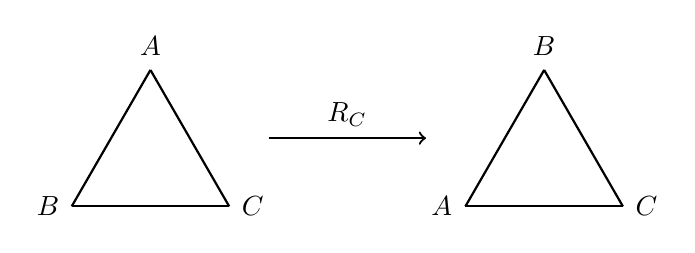
\begin{tikzpicture}
	\draw (1,2.032) node{$A$};
	\draw (-0.3,0) node{$B$};
	\draw (2.3,0) node{$C$};
	\draw (6,2.032) node{$B$};
	\draw (4.7,0) node{$A$};
	\draw (7.3,0) node{$C$};
	\draw (3.5,1.166) node{$R_C$};
	\draw[thick](0,0)--(1,1.732); 
	\draw[thick](0,0)--(2,0);
	\draw[thick](1,1.732)--(2,0);
	\draw[thick,->](2.5,0.866)--(4.5,0.866);
	\draw[thick](5,0)--(6,1.732);
	\draw[thick](5,0)--(7,0);
	\draw[thick](6,1.732)--(7,0);
\end{tikzpicture}
Where $R_\theta$ denotes a clockwise rotation about the center of the triangle by $\theta$ degrees while $R_A$ denotes the reflection through the plane of symmetry passing through $A$ which (obviously) is perpendicular to $\overline{BC}$.\\
So, in total, we have six symmetry elements for a planar equilateral triangle. Let us now study the composition of these symmetry elements.\\
Obviously $R_0$ composed with any symmetry element $\mathcal{S}$ should result in $\mathcal{S}$ and $R_\theta$ composed with $R_\alpha$ would result in $R_{\theta+\alpha}$. But $R_A\circ R_{120}$ results in $R_C$ whereas $R_{120}\circ R_A$ results in $R_B$. Representing all these in a tabular form, we obtain what is known as the Cayley table or more colloquially, a multiplication/operation table.\\
Note that for the table, the composition order is $(\text{column}\circ\text{row})$.
\begin{center}
\begin{tabular}{c|c c c c c c}
	  & $R_{0}$ & $R_{120}$ & $R_{240}$ & $R_{A}$ & $R_{B}$ & $R_{C}$\\
	  \hline
	  $R_0$ & $R_{0}$ & $R_{120}$ & $R_{240}$ & $R_{A}$ & $R_{B}$ & $R_{C}$\\
	  $R_{120}$ & $R_{120}$ & $R_{240}$ & $R_{0}$ & $R_C$ & $R_A$ & $R_B$\\
	  $R_{240}$ & $R_{240}$ & $R_0$ & $R_{120}$ & $R_B$ & $R_C$ & $R_A$\\
	  $R_A$ & $R_A$ & $R_B$ & $R_C$ & $R_0$ & $R_{120}$ & $R_{240}$\\
	  $R_B$ & $R_B$ & $R_C$ & $R_A$ & $R_{240}$ & $R_0$ & $R_{120}$\\
	  $R_C$ & $R_C$ & $R_A$ & $R_B$ & $R_{120}$ & $R_{240}$ & $R_0$\\
\end{tabular}
\end{center}

The above table shows us that the composition of any two symmetry elements gives another symmetry element. This property is called \textit{closure} which is a necessary property for a group. Also, note that $a\circ b$ need not be the same as $b\circ a$. But, in the case when $a\circ b=b\circ a$ for all elements $a$ and $b$, the group is said to be \textit{commutative} or a scarier term for the same is \textit{Abelian}\footnote{Named after Neils Henrik Abel}. Finally, one can check that $(a\circ b)\circ c=a\circ(b\circ c)$ for any three symmetry elements $a$, $b$ and $c$.\footnote{I shall leave the verification of this as an exercise for the reader} This property is called \textit{associativity} which is another necessary property for a group.\\

From the above discussion, we can conclude that the set of symmetries of a planar equilateral triangle forms a group.\footnote{This is a slight abuse of language, since a group needs a binary operator associated with it but we shall deal with this in the next chapter.} This group is denoted by $D_3$ and is called ``the dihedral group of order $6$". Note that the order of the group is determined by the number of elements. In general, $D_n$ is used to represent the set of symmetries of a planar $n$-gon. A natural question to ask at this point is whether the order of $D_n$ is $2n$ (which you may or may not have conjectured while dealing with $D_3$).\\
The answer is \textbf{yes}. It is rather easy to prove. Let us consider a general $n$-gon given by $A_1A_2\cdots A_n$. We are interested in the ``permissible permutations" of $A_1A_2\cdots A_n$. We note that any symmetry does not change the ``adjacency" of the vertices that is, in particular, $A_1$ and $A_2$ must be adjacent in all such permutations. Now, for all the permutations, $A_1$ can be placed in $n$ positions. Once the position of $A_1$ has been decided, there are only two valid placements of $A_2$. Once the positions of both $A_1$ and $A_2$ have been decided, the positions of all the vertices get determined. Thus, only $n\times2=2n$ symmetry elements are possible.




